\chapter{Collaborative Design}

\exercise{4.4}
See text.

\solution
\begin{enumerate}
	\item 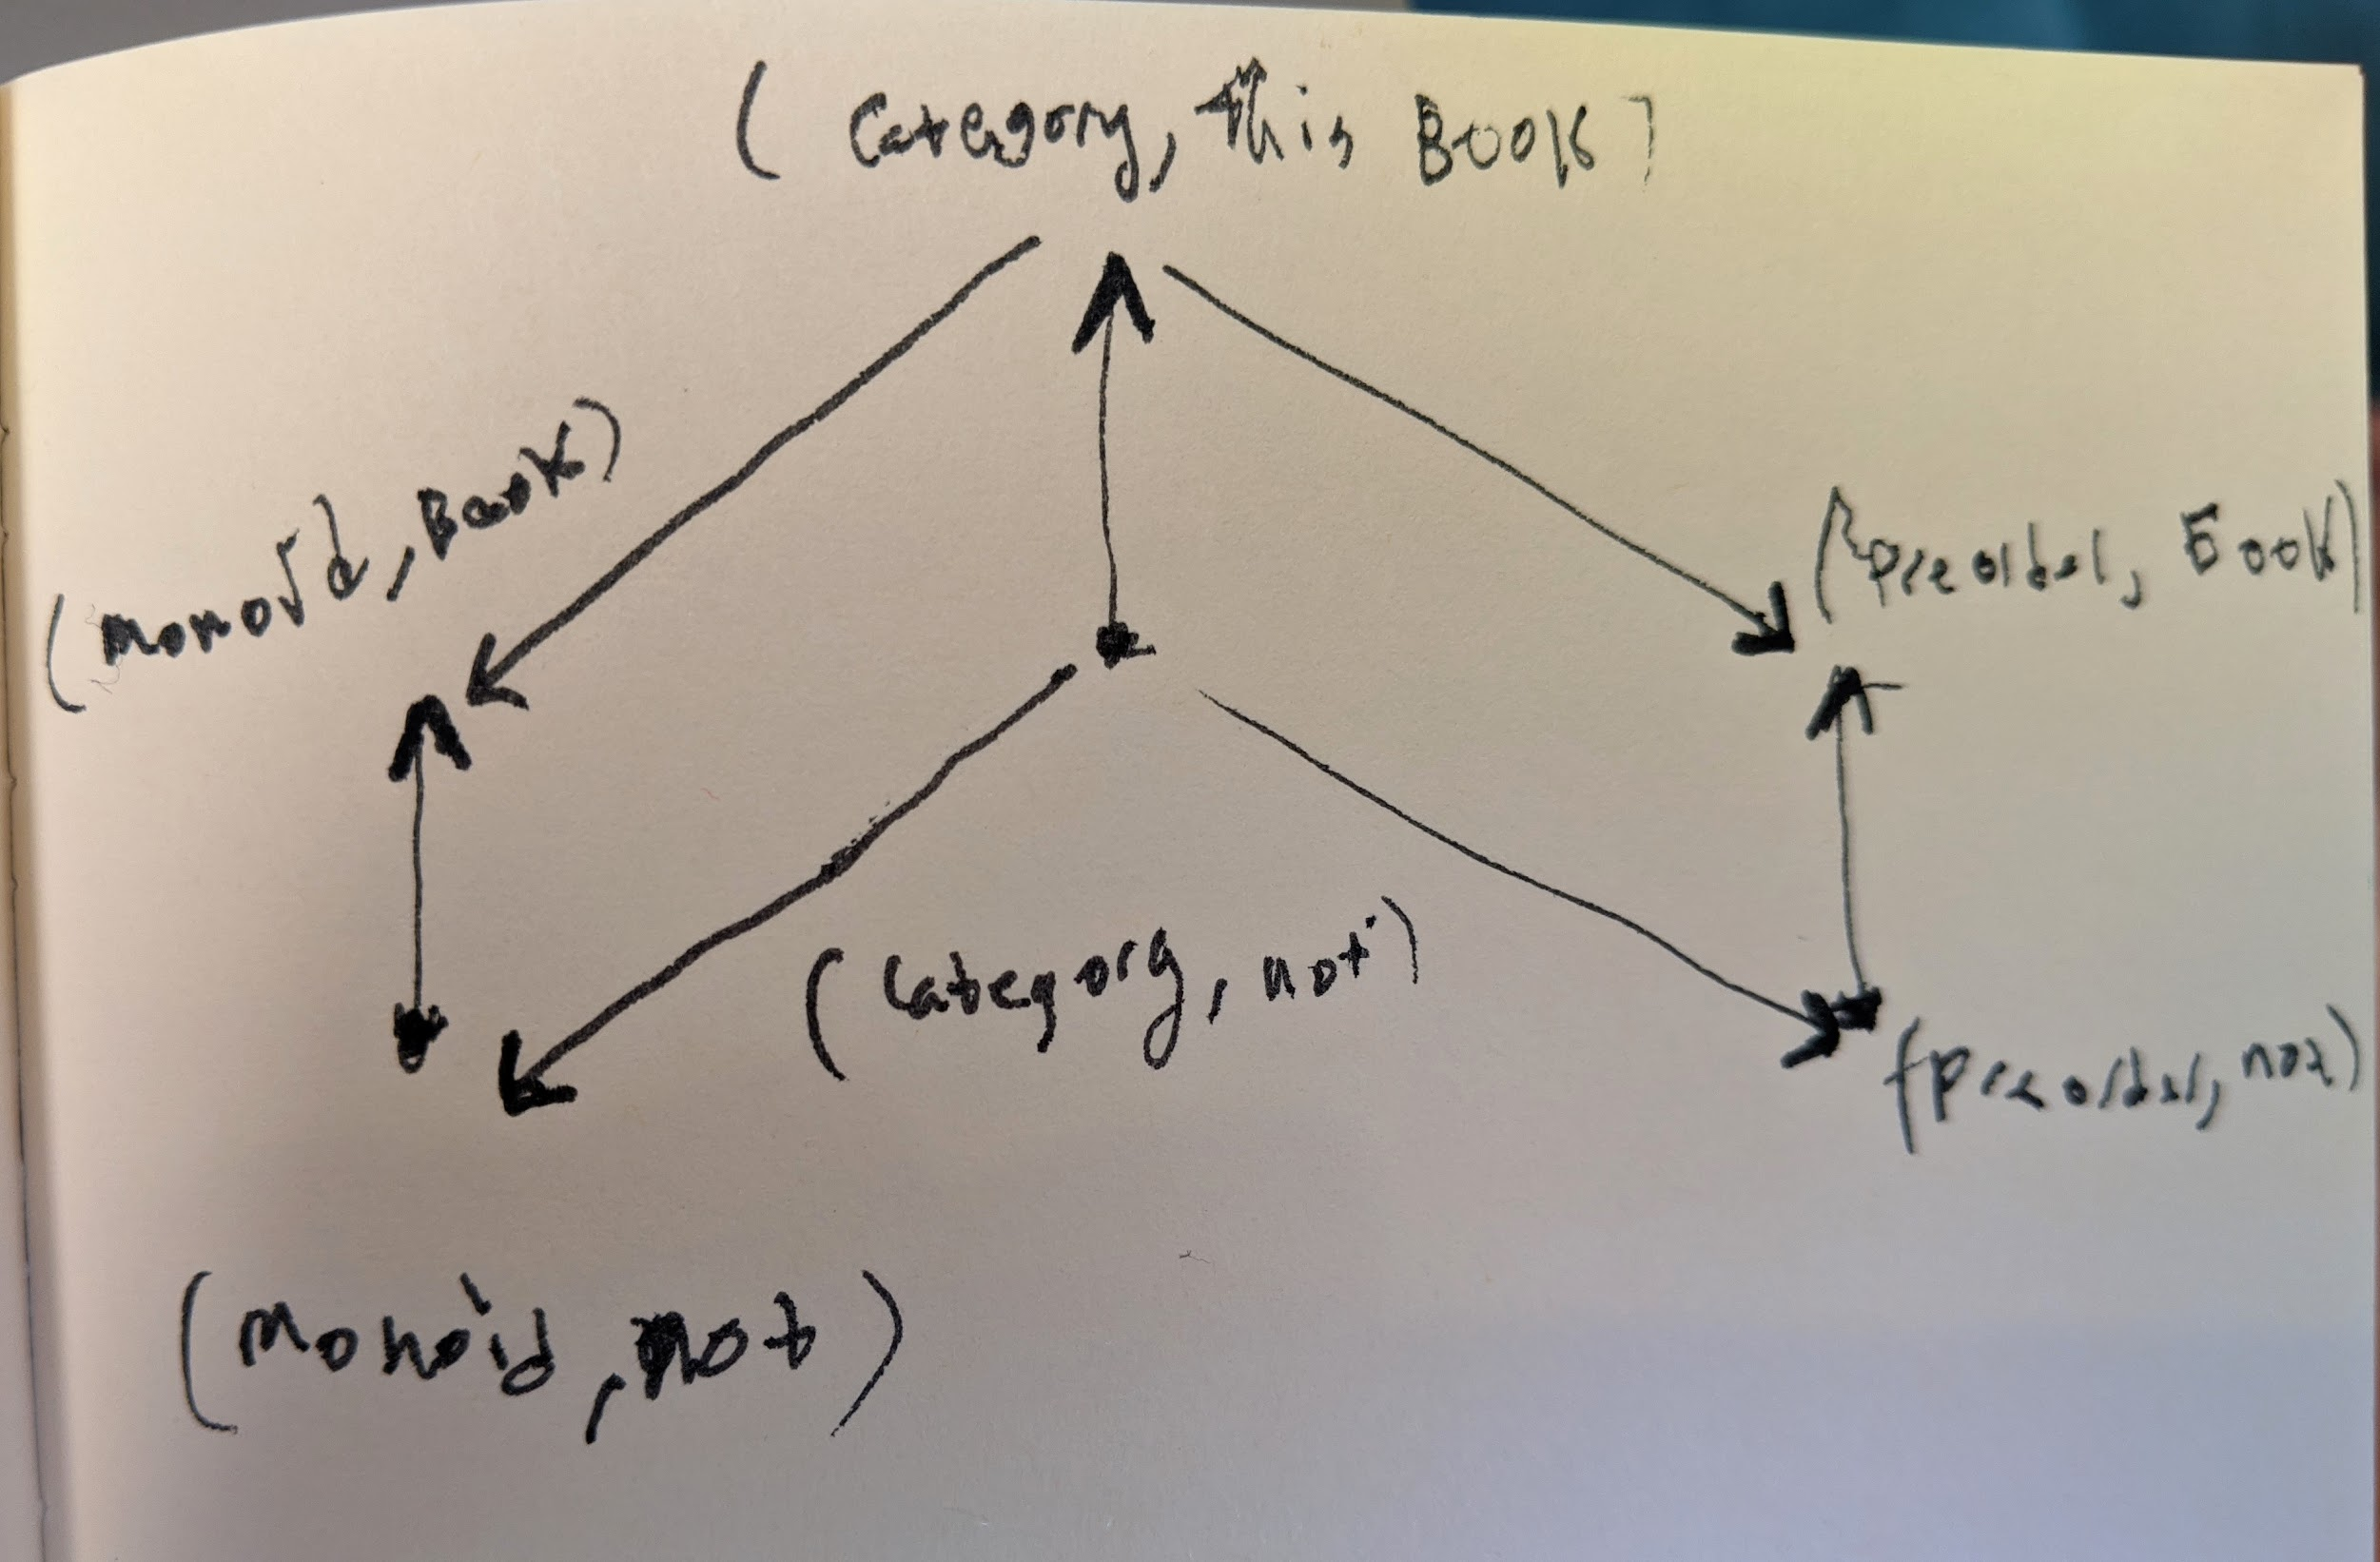
\includegraphics[width=0.5\textwidth]{images/4-4.jpg}
	\item $\Lambda(x,$ book) = true  and $\Lambda(x,$ nothing) = false for any $x\in\mcX$.
	
	  An interpretation of the fact that the preimage of true forms an upper set in $\mcX^\opp\times\mcY$ is that moving up in the product preorder corresponds to something easier, whether it is an easier topic to explain or more information to use to explain it.  So if your aunt can explain a preorder with nothing, she can definitely explain a preorder with this book, but not necessarily a category; and if she can explain a category with this book, she can definitely explain both a monoid and a preorder with this book, but not necessarily any of these topics with nothing.
\end{enumerate}

\exercise{4.7}
Discussed in person.

\exercise{4.9}
Show that a $\mcV$-profunctor is the same as a function $\Phi:\Ob(\mcX)\times\Ob(\mcY)\to V$ such that for any $x,x'\in\mcX$ and $y,y'\in\mcY$, the following holds in $\mcV$:
$$\mcX(x',x)\otimes\Phi(x,y)\otimes\mcY(y,y')\leq\Phi(x',y').$$

\solution
For a function $\Phi:\Ob(\mcX)\times\Ob(\mcY)\to \mcV$, let's use $C$ to refer to the condition \textit{for any $x,x'\in\mcX$ and $y,y'\in\mcY$, the following holds in $\mcV$:}
$$\mcX(x',x)\otimes\Phi(x,y)\otimes\mcY(y,y')\leq\Phi(x',y').$$

We first first note by the definition of a product $\mcV$-category, for any $x,x'\in\Ob(\mcX)$ and $y,y'\in\Ob(\mcY)$,
$$(\mcX^\opp\times\mcY)((x,y),(x',y'))=\mcX(x',x)\otimes\mcY(y,y')$$

So as the quantale monoid is commutative, we can see the $C$ is equivalent to \textit{for all $x,x'\in\mcX$ and $y,y'\in\mcY$, the following holds in $\mcV$:}
$$(\mcX^\opp\times\mcY)((x,y),(x',y'))\otimes\Phi(x,y)\leq\Phi(x',y').$$

Secondly we revisit the definition of a quantale enriched in itself, for $v,v'\in \mcV$ we denote $\mcV(v,v')$ as  $v\multimap v'$, and for any $t,w,v\in \mcV$
 $$(t\otimes v)\leq w \iff t\leq (v\multimap w)$$
 
Using this we can further rewrite $C$ as \textit{for all $x,x'\in\mcX$ and $y,y'\in\mcY$, the following holds in $\mcV$:}
$$(\mcX^\opp\times\mcY)((x,y),(x',y'))\leq\mcV(\Phi(x,y),\Phi(x',y')).$$

We now note this is precisely the definition of a $\mcV$-profunctor.

\exercise{4.10}
Discussed in person.

\exercise{4.12}
See text.

\solution
$$\begin{array}{c|ccccc}
\Phi & a & b & c & d & e \\
\hline N & \true & \false & \true & \false & \true \\
E & \true & \true & \false & \true & \false \\
W & \true & \false & \true & \false & \true \\
S & \true & \true & \true & \true & \true
\end{array}$$

\exercise{4.15}
See text.

\solution
$$\begin{array}{c|ccc}
\Phi & x & y & z \\
\hline A & 17 & 20 & 20 \\
B & 11 & 14 & 14 \\
C & 14 & 17 & 17 \\
D & 12 & 9 & 15
\end{array}$$

\exercise{4.17}
Calculate $M_X^3*M_\Phi*M_Y^2$, remembering to do matrix multiplication according to the $(\min,+)$-formula for matrix multiplication in the quantale $\Cost$.  Your answer should agree with the one you got in Exercise 4.15.

\solution
Discussed in person.

\exercise{4.18}
See text.

\solution
This is valid, it just means that it is not possible to make a good-natured funny movie even with \$1M, i.e. $\Phi(($g/n, funny$), $\$1M$)$ = false.

\exercise{4.22}
See text.

\solution
$$\begin{array}{c|cccc}
\Phi \fcmp \Psi & p & q & r & s \\
\hline A & 18 & 24 & 16 & 17 \\
B & 16 & 18 & 14 & 15 \\
C & 19 & 21 & 17 & 18 \\
D & 11 & 13 & 9 & 10
\end{array}$$

\exercise{4.26}
Choose a $\Cost$-category $\mcX$.  Give a bridge-style diagram for the unit profunctor $U_\mcX:\mcX\to\mcX$.

\solution
Discussed in person; there will be a bridge between each object and itself with cost 0.

\exercise{4.30}
Justify the steps in the proof of Lemma 4.27, and show which inequalities are actually equalities in the case where $\mcV=\Bool$.

\solution

\exercise{4.32}
Prove that composition of profunctors is associative.

\solution






